\chapter{Model Bisnis Platform dan Efek Jaringan}
\label{ch:ch02}

\section*{Tujuan Pembelajaran}
\begin{itemize}
  \item Mengidentifikasi sisi pasar, interaksi inti, dan nilai bagi tiap sisi pada sebuah platform.
  \item Membedakan efek jaringan sisi sama dan lintas sisi, baik yang positif maupun yang negatif.
  \item Menganalisis strategi mengatasi masalah ayam dan telur (\textit{chicken-and-egg problem}) saat platform diluncurkan.
\end{itemize}

\section{Pendahuluan}

Pada rapat awal program ``Satu Pasien, Satu Rekam Medis'', direksi Medikara
Health sepakat membuka aplikasi Medikara+ bagi klinik mitra dan perusahaan
asuransi. Kesepakatan itu langsung memunculkan pertanyaan yang tidak dapat
dijawab oleh tim teknologi. Klinik mitra mau bergabung bila pasiennya banyak,
sedangkan pasien mau memakai aplikasi bila pilihan dokternya banyak. Tim
pemasaran mengusulkan layanan gratis bagi pasien. Tim keuangan meminta klinik
mitra membayar biaya langganan. Perusahaan asuransi bertanya apa untungnya bagi
mereka.

Pertanyaan semacam itu adalah pertanyaan model bisnis platform. Bab 1 sudah
membedakan bisnis \textit{pipeline}, yang membuat lalu menjual, dengan bisnis
platform, yang mempertemukan beberapa pihak dan memudahkan interaksi di antara
mereka. Bab ini membuka mesin di balik platform. Bahasannya meliputi siapa saja
sisi pasarnya, interaksi apa yang menjadi alasan platform ada, bagaimana efek
jaringan membuat platform tumbuh atau runtuh, bagaimana platform baru keluar
dari masalah ayam dan telur, siapa yang sebaiknya membayar, dan kapan model
platform justru tidak cocok. Ekosistem mitra yang lebih luas beserta pilihan
membangun, bergabung, atau bermitra dibahas di Bab 3.

Rujukan utama bab ini adalah buku \textit{Platform Revolution}
\cite{parker2016platform} dan \textit{The Business of Platforms}
\cite{cusumano2019business}. Definisi platform multi-sisi diambil dari Hagiu dan
Wright \cite{hagiu2015multisided}. Teori harga pasar dua sisi diambil dari
Rochet dan Tirole \cite{rochet2003platform} serta Parker dan Van Alstyne
\cite{parker2005twosided}. Panduan strategi praktisnya diambil dari Eisenmann,
Parker, dan Van Alstyne \cite{eisenmann2006strategies}.

\IfFileExists{../figures/ch02-diagram-konsep.png}{%

Gambar \ref{fig:ch02-ilustrasi-bab} merangkum hubungan komponen dan konsep utama bab ini.
\begin{figure}[!htb]
  \centering
  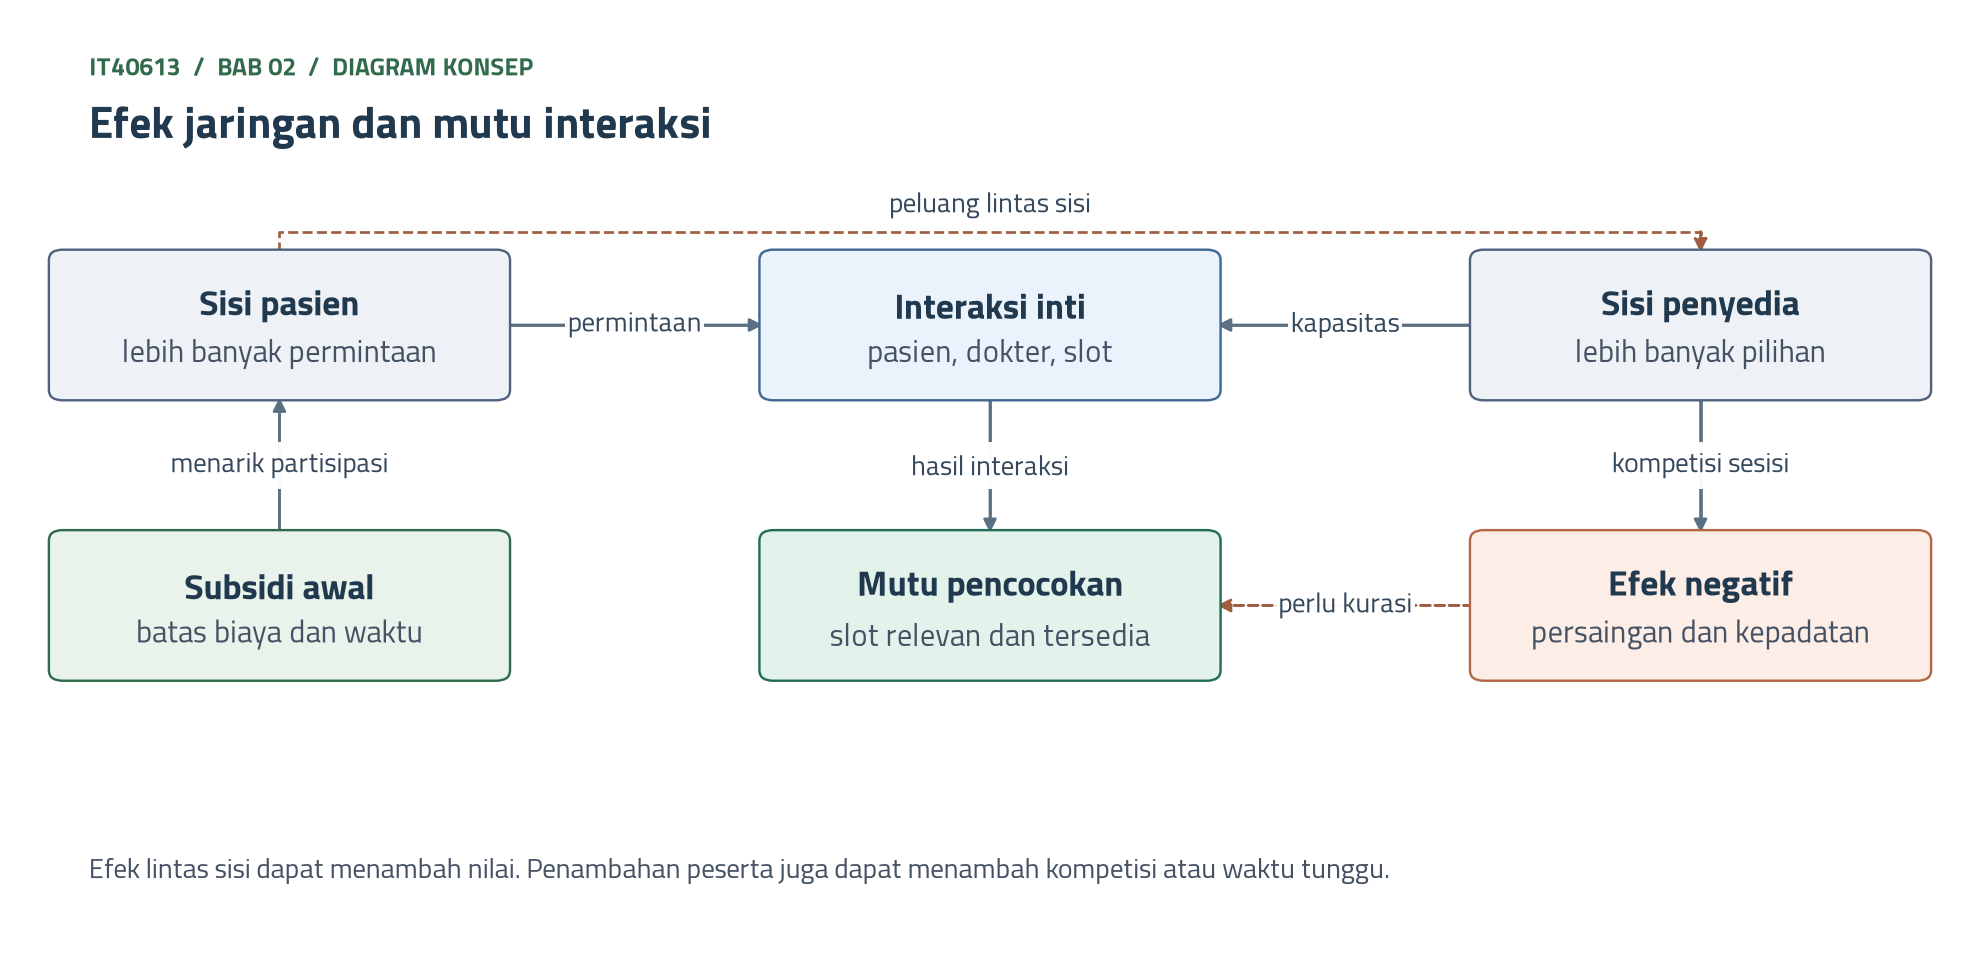
\includegraphics[width=\textwidth]{../figures/ch02-diagram-konsep.png}
  \caption{Efek jaringan dan mutu interaksi}
  \label{fig:ch02-ilustrasi-bab}
\end{figure}
}{}

\section{Pasar Dua Sisi dan Pasar Multi-Sisi}

Setiap hari ribuan pasien datang ke lima rumah sakit dan 18 klinik Medikara
untuk bertemu dokter. Sekilas Medikara sudah mempertemukan dua pihak, yaitu
pasien dan dokter. Pertanyaannya, apakah itu berarti Medikara sudah menjadi
platform? Jawabannya belum. Alasannya terletak pada siapa yang memegang kendali
atas pertemuan itu.

Hagiu dan Wright mendefinisikan platform multi-sisi sebagai organisasi yang
menciptakan nilai terutama dengan memungkinkan interaksi langsung antara dua
jenis pelanggan atau lebih, dan setiap jenis pelanggan itu berafiliasi dengan
platform \cite{hagiu2015multisided}. Definisi ini memuat dua syarat. Syarat
pertama adalah interaksi langsung: kedua sisi memegang kendali atas syarat
utama interaksi, misalnya harga, isi layanan, dan cara penyerahannya. Syarat
kedua adalah afiliasi: setiap sisi dengan sadar bergabung ke platform, misalnya
mendaftar, membayar biaya keanggotaan, atau menyiapkan diri agar dapat dilayani
lewat platform. Pasar dua sisi adalah bentuk paling sederhana dengan dua jenis
pelanggan. Pasar multi-sisi melibatkan tiga jenis atau lebih.

Kedua syarat itu memisahkan platform dari dua model lain yang sering tertukar.
Pengecer membeli barang, lalu menjualnya kembali dengan harga dan syarat yang
ditentukannya sendiri, sehingga pemasok dan pembeli tidak berinteraksi
langsung. Perusahaan \textit{pipeline} memakai pemasok atau tenaga kerja,
tetapi pihak itu tidak berafiliasi dengan pelanggan akhir. Tabel
\ref{tab:ch02-tiga-model} merangkum perbedaannya.

\begin{table}[!htb]
  \centering
  \caption{Pengecer, \textit{pipeline}, dan platform multi-sisi dibedakan oleh
           kendali atas syarat interaksi dan oleh afiliasi}
  \label{tab:ch02-tiga-model}
  \begin{tabularx}{\textwidth}{lXX}
    \hline
    \textbf{Model} & \textbf{Penentu harga dan syarat} & \textbf{Contoh layanan kesehatan} \\
    \hline
    Pengecer & Pengecer sendiri; pemasok tidak berhubungan dengan pembeli & Apotek yang membeli obat dari distributor lalu menjualnya \\
    \hline
    \textit{Pipeline} & Perusahaan; tenaga kerja tidak berafiliasi dengan pelanggan & Rumah sakit yang menggaji dokter dan menetapkan tarif \\
    \hline
    Platform multi-sisi & Kedua sisi; keduanya mendaftar ke platform & Aplikasi tempat dokter menetapkan jadwal dan tarif sendiri \\
    \hline
  \end{tabularx}
\end{table}

Bedanya mirip toko kelontong dan pengelola pasar tradisional. Pemilik toko
kelontong membeli beras dari distributor, menentukan harga jual, lalu melayani
pembeli. Pengelola pasar tidak membeli beras sama sekali. Ia menyewakan lapak,
menjaga kebersihan, dan mengatur parkir, sedangkan pedagang dan pembeli
menawar harga sendiri. Pembeli datang karena pedagangnya banyak, dan pedagang
menyewa lapak karena pembelinya ramai.

Dua contoh dari Medikara memperjelas bedanya:
\begin{enumerate}
  \item Rumah sakit Medikara di Bekasi mempekerjakan dokter, menetapkan tarif
        konsultasi spesialis Rp250.000, dan menagih pasien atas nama rumah
        sakit. Pasien bertransaksi dengan rumah sakit, bukan langsung dengan
        dokter. Model ini adalah \textit{pipeline}, walaupun pasien dan dokter
        bertemu setiap hari.
  \item Misalkan Medikara+ membuka jadwal bagi 40 klinik pratama mitra. Setiap
        klinik menetapkan tarifnya sendiri, misalnya antara Rp90.000 dan
        Rp150.000 per konsultasi, mengatur jadwal dokternya, dan menerima
        pembayaran pasien lewat aplikasi. Medikara+ hanya menyediakan tempat
        bertemu, sistem pemesanan, dan pembayaran. Bagian layanan ini memenuhi
        kedua syarat, sehingga Medikara+ bekerja sebagai platform.
\end{enumerate}

Platform sendiri tidak seragam. Cusumano, Gawer, dan Yoffie membaginya menjadi
dua jenis dasar \cite{cusumano2019business}. Platform transaksi menjadi
perantara yang memudahkan pertukaran barang, jasa, atau informasi antara
pihak-pihak yang sulit bertemu tanpanya, misalnya \textit{marketplace} dan
transportasi daring. Platform inovasi menjadi fondasi tempat pihak ketiga
membangun produk pelengkap, misalnya sistem operasi ponsel yang memungkinkan
pengembang luar membuat aplikasi. Perusahaan yang menjalankan keduanya sekaligus
disebut platform hibrida. Medikara+ pada tahap awal adalah platform transaksi.
Medikara+ baru menjadi platform inovasi bila Medikara membuka
\textit{Application Programming Interface} (API) agar pihak lain membangun
layanan di atasnya, misalnya aplikasi kesehatan karyawan milik perusahaan
klien. Topik itu muncul lagi di Bab 3 dan Bab 4.

Gambar \ref{fig:ch02-sisi-pasar} memperlihatkan calon sisi pasar Medikara+.
Dua sisi berwarna oranye membentuk interaksi inti, sedangkan tiga sisi
berwarna biru adalah calon sisi tambahan.

\begin{figure}[!htb]
  \centering
  \begin{tikzpicture}[
  font=\scriptsize,
  kotak/.style={draw, rounded corners, minimum height=0.95cm, minimum width=2.5cm,
                align=center, font=\scriptsize\bfseries},
  panah/.style={-{Stealth[length=2mm]}, thick},
  duaarah/.style={{Stealth[length=2mm]}-{Stealth[length=2mm]}, thick},
  ket/.style={font=\tiny, align=center, fill=white, inner sep=1.5pt}
]
  \node[kotak, fill=praditagreen!15, minimum width=2.7cm, minimum height=1.1cm] (inti)
    at (0,0) {Medikara+\\{\tiny\mdseries platform}};

  \node[kotak, fill=orange!12] (pasien) at (-4.6,0)
    {Pasien\\{\tiny\mdseries mencari dan memesan}};
  \node[kotak, fill=orange!12] (dokter) at (4.6,0)
    {Dokter klinik mitra\\{\tiny\mdseries membuka jadwal}};
  \node[kotak, fill=blue!8] (perusahaan) at (-2.4,2.0)
    {Perusahaan klien\\{\tiny\mdseries layanan karyawan}};
  \node[kotak, fill=blue!8] (asuransi) at (2.4,2.0)
    {Asuransi swasta\\{\tiny\mdseries penjaminan biaya}};
  \node[kotak, fill=blue!8, minimum width=3.4cm] (apotek) at (0,-2.75)
    {Apotek dan laboratorium mitra\\{\tiny\mdseries resep dan hasil pemeriksaan}};

  \draw[duaarah] (pasien) -- node[ket, above] {cari, pesan, bayar} (inti);
  \draw[duaarah] (dokter) -- node[ket, above] {jadwal, layanan} (inti);
  \draw[duaarah] (perusahaan) -- (inti);
  \draw[duaarah] (asuransi) -- (inti);
  \draw[duaarah] (apotek) -- (inti);

  % Busur dilandaikan agar tidak menyentuh kotak apotek, dan labelnya di luar panah tengah.
  \draw[panah, dashed, gray!70!black] (pasien.south) to[out=-40, in=-140, looseness=0.6]
    node[ket, below, pos=0.2, xshift=-4pt] {interaksi langsung:\\janji temu dan konsultasi}
    (dokter.south);

  \node[font=\tiny, anchor=north, align=center, text=gray!60!black] at (0,-3.4)
    {oranye: sisi interaksi inti \quad biru: calon sisi tambahan};
\end{tikzpicture}

  \caption{Calon sisi pasar Medikara+. Garis putus-putus menandai interaksi
           langsung antara pasien dan dokter klinik mitra}
  \label{fig:ch02-sisi-pasar}
\end{figure}

\begin{kasus}[title={Kasus Medikara Health: Siapa Sisi Pasar Medikara+?}]
Tim strategi Medikara mendaftar tujuh calon pihak, lalu mengujinya dengan dua
syarat Hagiu dan Wright.

Pasien dan dokter klinik mitra jelas memenuhi kedua syarat. Pasien mendaftar,
memilih dokter, dan membayar. Dokter klinik mitra mendaftar, menetapkan jadwal
dan tarif, lalu melayani. Keduanya membentuk interaksi inti.

Dokter internal berada di wilayah abu-abu. Tarif tatap mukanya ditetapkan
Medikara, sehingga untuk layanan tatap muka mereka bagian dari
\textit{pipeline}. Namun keikutsertaan mereka di telekonsultasi bersifat
sukarela dan honornya dihitung per konsultasi. Karena itu perilakunya mirip
sisi pasar: mereka membuka jadwal daring bila pasiennya cukup.

Asuransi swasta, perusahaan klien, serta apotek dan laboratorium mitra menjadi
sisi bila masing-masing mendaftar dan bertransaksi langsung lewat Medikara+.
Contohnya verifikasi penjaminan per pemesanan, paket layanan bagi karyawan,
serta pengiriman resep dan hasil pemeriksaan. Ketiganya ditunda sampai interaksi
inti berjalan.

Badan Penyelenggara Jaminan Sosial (BPJS) Kesehatan tidak diperlakukan sebagai
sisi pasar. Tarif dan aturan klaim program Jaminan Kesehatan Nasional tidak
dirundingkan lewat Medikara+. Hubungan dengan BPJS Kesehatan tetap berupa
integrasi wajib yang dibahas di Bab 7.
\end{kasus}

\section{Interaksi Inti: Partisipan, Unit Nilai, dan Filter}

Daftar sisi pasar belum menjawab pertanyaan yang lebih mendasar: interaksi apa
yang membuat orang datang ke Medikara+? Tanpa jawaban yang tajam, tim produk
cenderung menambah fitur apa saja yang diminta. Aplikasinya lalu menjadi
etalase menu yang jarang dipakai.

Parker, Van Alstyne, dan Choudary menyebut pertukaran nilai terpenting pada
sebuah platform sebagai interaksi inti (\textit{core interaction})
\cite{parker2016platform}. Interaksi inti punya tiga unsur. Partisipan adalah
pihak yang terlibat, yaitu produsen yang menciptakan nilai dan konsumen yang
memakainya; satu orang dapat bergantian memainkan kedua peran. Unit nilai
(\textit{value unit}) adalah informasi yang ditawarkan produsen, misalnya
daftar barang, posisi pengemudi, atau slot jadwal dokter. Filter adalah aturan
atau algoritma yang menentukan unit nilai mana yang sampai ke konsumen
tertentu. Agar interaksi inti terjadi berulang kali, platform menjalankan tiga
fungsi: menarik (\textit{pull}) partisipan, memudahkan (\textit{facilitate})
interaksi, dan mencocokkan (\textit{match}) produsen dengan konsumen yang
tepat. Gambar \ref{fig:ch02-interaksi-inti} memperlihatkan alurnya pada
Medikara+.

\begin{figure}[!htb]
  \centering
  \begin{tikzpicture}[
  font=\scriptsize,
  kotak/.style={draw, rounded corners, minimum height=1.25cm, text width=2.15cm,
                align=center, font=\scriptsize\bfseries},
  fungsi/.style={draw, rounded corners, minimum height=0.6cm, minimum width=2.0cm,
                 align=center, fill=praditagreen!15, font=\scriptsize\bfseries},
  panah/.style={-{Stealth[length=2mm]}, thick},
  garis/.style={dashed, gray!70!black}
]
  \node[kotak, fill=blue!8] (produsen) at (0,0)
    {Produsen\\{\tiny\mdseries dokter yang membuka jadwal}};
  \node[kotak, fill=blue!8] (unit) at (2.9,0)
    {Unit nilai\\{\tiny\mdseries slot jadwal, profil, tarif}};
  \node[kotak, fill=orange!12] (filter) at (5.8,0)
    {Filter\\{\tiny\mdseries spesialisasi, lokasi, penjamin}};
  \node[kotak, fill=blue!8] (konsumen) at (8.7,0)
    {Konsumen\\{\tiny\mdseries pasien yang mencari}};
  \node[kotak, fill=green!10, text width=3.2cm] (interaksi) at (7.25,-2.1)
    {Interaksi terjadi\\{\tiny\mdseries janji temu atau konsultasi}};

  \draw[panah] (produsen) -- (unit);
  \draw[panah] (unit) -- (filter);
  \draw[panah] (filter) -- (konsumen);
  % Kedua panah tegak lurus terhadap kotak interaksi, supaya tidak masuk ke dalam kotak.
  \draw[panah] (konsumen.south) -- (konsumen.south |- interaksi.north);
  \draw[panah] (filter.south |- interaksi.north) --
    node[font=\tiny, align=right, midway, left]
    {ulasan dan data kunjungan\\memperbaiki filter} (filter.south);

  \node[fungsi] (tarik) at (1.45,1.55) {Menarik};
  \node[fungsi] (mudah) at (4.35,1.55) {Memudahkan};
  \node[fungsi] (cocok) at (7.25,1.55) {Mencocokkan};
  \draw[garis] (tarik.south) -- (produsen.north);
  \draw[garis] (tarik.south) -- (unit.north);
  \draw[garis] (mudah.south) -- (unit.north);
  \draw[garis] (mudah.south) -- (filter.north);
  \draw[garis] (cocok.south) -- (filter.north);
  \draw[garis] (cocok.south) -- (konsumen.north);
  \node[font=\tiny, text=gray!60!black, anchor=south] at (4.35,1.95)
    {tiga fungsi platform};
\end{tikzpicture}

  \caption{Interaksi inti pemesanan janji temu di Medikara+. Filter ditekankan
           karena di sanalah platform menambah nilai paling besar}
  \label{fig:ch02-interaksi-inti}
\end{figure}

Cara kerjanya mirip papan lowongan di bursa kerja kampus. Perusahaan
menempelkan lowongan, yaitu unit nilainya. Mahasiswa datang untuk membaca,
yaitu konsumennya. Petugas bursa kerja memilah lowongan menurut jurusan dan
menempelkannya di papan yang berbeda, yaitu filternya. Bila papan penuh dengan
lowongan yang tidak relevan, mahasiswa berhenti datang walaupun jumlah
lowongannya banyak.

Dua contoh berikut memperlihatkan peran filter:
\begin{enumerate}
  \item Misalkan Medikara+ menampilkan 1.400 slot jadwal per hari dari sekitar 640
        dokter di seluruh fasilitas. Tanpa filter, seorang ibu di Depok yang
        mencari dokter anak harus menggulir ratusan slot yang tidak relevan.
        Dengan filter spesialisasi, lokasi dalam radius 10 km, dan penjamin
        yang dimilikinya, pilihannya menyusut menjadi 18 slot. Dari 18 slot itu
        ia dapat memutuskan dalam satu menit.
  \item Filter yang buruk merusak kepercayaan. Misalkan filter hanya
        mengurutkan dokter menurut jumlah ulasan. Dokter yang sudah lama
        bergabung selalu tampil teratas dan jadwalnya penuh sampai tiga minggu,
        sedangkan dokter baru dengan jadwal kosong hampir tidak pernah
        terlihat. Pasien menunggu lebih lama, dokter baru pergi, dan platform
        kehilangan produsen yang justru dibutuhkan.
\end{enumerate}

Tabel \ref{tab:ch02-interaksi-inti} membandingkan unsur interaksi inti pada
beberapa platform yang dikenal di Indonesia.

\begin{table}[!htb]
  \centering
  \caption{Unsur interaksi inti pada empat jenis platform}
  \label{tab:ch02-interaksi-inti}
  \begin{tabularx}{\textwidth}{lllX}
    \hline
    \textbf{Platform} & \textbf{Produsen} & \textbf{Unit nilai} & \textbf{Filter} \\
    \hline
    Transportasi daring & Pengemudi & Posisi pengemudi & Jarak, arah, jenis kendaraan \\
    \hline
    \textit{Marketplace} & Penjual & Daftar produk & Kata kunci, lokasi gudang, reputasi \\
    \hline
    Telekonsultasi & Dokter & Slot konsultasi & Spesialisasi, jam praktik, tarif \\
    \hline
    Janji temu Medikara+ & Dokter & Slot tatap muka & Lokasi, penjamin, waktu tunggu \\
    \hline
  \end{tabularx}
\end{table}

\begin{kasus}[title={Kasus Medikara Health: Memilih Interaksi Inti Medikara+}]
Medikara+ saat ini punya dua layanan utama, yaitu pemesanan janji temu dan
telekonsultasi. Tim produk perlu memilih salah satu sebagai interaksi inti.

Bab 1 mencatat sekitar 28.000 janji temu per bulan lewat Medikara+, yaitu 336.000
per tahun, atau sekitar 28\% dari 1,2 juta kunjungan. Telekonsultasi melayani 6.000
pasien aktif per bulan dengan rata-rata 0,3 konsultasi per pasien, yaitu 1.800
konsultasi per bulan atau 21.600 per tahun. Dari sisi volume, janji temu sekitar
lima belas kali lebih besar, sehingga janji temu dipilih sebagai interaksi inti.
Telekonsultasi menjadi interaksi pendukung.

Pilihan ini membawa satu konsekuensi teknis. Unit nilai janji temu, yaitu slot
jadwal, disimpan di lima Sistem Informasi Manajemen Rumah Sakit (SIMRS) dengan
versi berbeda. Bab 1 mencatat data slot diperbarui ke Medikara+ setiap lima menit.
Misalkan 1\% pemesanan, atau 280 per bulan, ternyata bentrok dengan pasien yang
mendaftar langsung di loket. Interaksi inti yang terlihat sederhana bagi pasien ternyata bergantung
pada integrasi yang rapuh. Integrasi ini dipotret di Bab 4 dan Bab 5.
\end{kasus}

\section{Efek Jaringan}

Aplikasi telekonsultasi yang sudah ramai sulit disaingi, sedangkan aplikasi
baru dengan fitur lebih lengkap sering tetap sepi. Penjelasannya ada pada efek
jaringan.

Efek jaringan (\textit{network effect}) terjadi ketika nilai platform bagi
seorang pengguna berubah karena jumlah pengguna lain
\cite{parker2016platform}. Efek sisi sama, disebut juga efek langsung, terjadi
di antara pengguna pada sisi yang sama. Contohnya pemain gim yang mendapat
lebih banyak kawan bermain ketika pemain lain bertambah. Efek lintas sisi,
disebut juga efek tidak langsung, terjadi di antara dua sisi. Contohnya pembeli
yang lebih tertarik pada \textit{marketplace} dengan banyak penjual, dan
sebaliknya. Keduanya dapat positif atau negatif. Eisenmann dan rekan mencatat
bahwa efek lintas sisi biasanya positif tetapi dapat negatif, misalnya penonton
televisi yang lebih suka iklan sedikit. Efek sisi sama justru sering negatif,
misalnya penjual yang lebih suka pesaingnya sedikit
\cite{eisenmann2006strategies}.

Pasar malam memperlihatkan keempatnya sekaligus. Pedagang yang banyak menarik
pengunjung, dan pengunjung yang ramai menarik pedagang. Pengunjung juga senang
datang bersama tetangga. Namun bila pengunjung terlalu padat, orang sulit
berjalan dan antre lama di setiap gerobak. Pedagang martabak kelima di lorong
yang sama juga harus membagi pembeli dengan empat pedagang lainnya.

Gambar \ref{fig:ch02-efek-jaringan} memetakan efek jaringan utama Medikara+,
sedangkan Tabel \ref{tab:ch02-jenis-efek} memberi contoh keempat jenisnya pada
layanan kesehatan beserta cara mengendalikannya.

\begin{figure}[!htb]
  \centering
  \begin{tikzpicture}[
  font=\scriptsize,
  kotak/.style={draw, rounded corners, minimum height=1.2cm, minimum width=2.4cm,
                align=center, font=\scriptsize\bfseries, fill=blue!8},
  panah/.style={-{Stealth[length=2mm]}, thick},
  positif/.style={draw, rounded corners=2pt, fill=green!10, font=\tiny,
                  align=center, inner sep=2pt},
  negatif/.style={draw, rounded corners=2pt, fill=red!22, font=\tiny,
                  align=center, inner sep=2pt}
]
  \node[kotak] (pasien) at (0,0) {Pasien\\{\tiny\mdseries sisi konsumen}};
  \node[kotak] (dokter) at (6.4,0) {Dokter\\{\tiny\mdseries sisi produsen}};

  \draw[panah] (dokter.north west) to[out=150, in=30]
    node[positif, above, yshift=2pt] {lintas sisi, positif:\\
      makin banyak dokter, makin banyak pilihan dan slot}
    (pasien.north east);
  \draw[panah] (pasien.south east) to[out=-30, in=-150]
    node[positif, below, yshift=-2pt] {lintas sisi, positif:\\
      makin banyak pasien, makin banyak konsultasi}
    (dokter.south west);

  \draw[panah, red!60!black] (pasien.north west) to[out=150, in=210, looseness=4.5]
    (pasien.south west);
  \node[negatif, anchor=north, text width=2.5cm] at (-1.3,-0.95)
    {sisi sama, negatif:\\slot cepat habis, antrean naik};

  \draw[panah, red!60!black] (dokter.north east) to[out=30, in=-30, looseness=4.5]
    (dokter.south east);
  \node[negatif, anchor=north, text width=2.5cm] at (7.7,-0.95)
    {sisi sama, negatif:\\dokter berebut pasien yang sama};
\end{tikzpicture}

  \caption{Peta efek jaringan Medikara+. Hijau menandai efek positif dan merah
           menandai efek negatif}
  \label{fig:ch02-efek-jaringan}
\end{figure}

\begin{table}[!htb]
  \centering
  \caption{Empat jenis efek jaringan pada platform layanan kesehatan}
  \label{tab:ch02-jenis-efek}
  \begin{tabularx}{\textwidth}{lXX}
    \hline
    \textbf{Jenis} & \textbf{Contoh} & \textbf{Cara menjaga atau mengendalikan} \\
    \hline
    Sisi sama, positif & Ulasan pasien membantu pasien lain memilih dokter & Hanya pasien yang benar-benar berkunjung boleh menulis ulasan \\
    \hline
    Sisi sama, negatif & Slot dokter favorit cepat habis ketika pasien bertambah & Batas pemesanan aktif per pasien dan daftar tunggu \\
    \hline
    Lintas sisi, positif & Makin banyak dokter, makin pendek waktu tunggu pasien & Rekrutmen dokter yang diarahkan ke spesialisasi yang kurang \\
    \hline
    Lintas sisi, negatif & Iklan produk kesehatan dari mitra mengganggu pasien & Batas jumlah iklan dan kurasi isi \\
    \hline
  \end{tabularx}
\end{table}

Dua contoh berangka memperlihatkan arah efek itu:
\begin{enumerate}
  \item Misalkan dokter telekonsultasi bertambah dari 60 menjadi 120. Waktu
        tunggu rata-rata konsultasi spesialis turun dari 5 hari menjadi 2
        hari. Pasien yang menyelesaikan pemesanan naik dari 55\% menjadi 70\%
        dari pasien yang membuka halaman jadwal. Kenaikan ini adalah efek
        lintas sisi positif: pasien mendapat nilai lebih karena sisi dokter
        tumbuh.
  \item Misalkan pada Senin pagi pasien yang membuka aplikasi naik tiga kali
        lipat, sedangkan jumlah dokter tetap. Slot hari itu habis pukul 07.30,
        dan keluhan ke pusat layanan naik dari 40 menjadi 130 per hari. Ini
        adalah efek sisi sama negatif: setiap pasien tambahan mengurangi nilai
        bagi pasien lain.
\end{enumerate}

Jumlah bukan satu-satunya penentu. Mutu interaksi sama pentingnya. Platform
dengan 1.000 dokter yang sebagian izin praktiknya belum diverifikasi lebih
berbahaya daripada platform dengan 200 dokter yang seluruhnya terverifikasi.
Karena itu, pertumbuhan yang mengorbankan kurasi dapat membalik efek jaringan
positif menjadi negatif.

\subsection{Efek Jaringan Lokal dan Global}

Zhu dan Iansiti menunjukkan bahwa skala saja tidak menjamin platform bertahan
\cite{c02-zhu2019platforms}. Struktur jaringannya ikut menentukan. Jaringan
yang terpecah menjadi banyak kelompok lokal lebih mudah diserang pesaing lokal,
karena pesaing cukup menang di satu kota tanpa harus menandingi jaringan
nasional. Pengemudi transportasi daring di Bandung tidak berguna bagi penumpang
di Bekasi, sehingga efek jaringannya bersifat lokal.

Janji temu tatap muka juga bersifat lokal. Pasien di Bogor jarang memilih dokter
anak di Bandung. Telekonsultasi lebih global, karena dokter di Bandung dapat
melayani pasien di Bekasi. Akibatnya, untuk janji temu yang dihitung adalah
kepadatan per kota, bukan jumlah total.

\subsection{Data sebagai Sumber Efek Jaringan}

Gregory dan rekan memperkenalkan efek jaringan data (\textit{data network
effect}): platform makin bernilai bagi setiap pengguna ketika platform makin
banyak belajar dari data yang dikumpulkannya \cite{c02-gregory2021data}. Pada
Medikara+, data kunjungan dapat memperbaiki perkiraan waktu tunggu dan
rekomendasi dokter. Namun data kesehatan termasuk data pribadi yang bersifat
spesifik menurut Pasal 4 ayat (2) Undang-Undang (UU) Nomor 27 Tahun 2022 tentang
Pelindungan Data Pribadi (UU PDP) \cite{uu27-2022-pdp}. Pemrosesannya menuntut
dasar hukum dan perlindungan yang lebih ketat. Rinciannya dibahas di IT40813 IT
Governance, Risk \& Compliance.

\begin{kasus}[title={Kasus Medikara Health: Lima Kota, Lima Jaringan Kecil}]
Misalkan dari sekitar 640 dokter Medikara, hanya 52 yang berpraktik di Bogor, dan hanya
empat di antaranya dokter anak. Bagi orang tua di Bogor, Medikara+ terasa sepi,
walaupun secara nasional jumlah dokternya terlihat besar. Pesaing yang punya 15
dokter anak di Bogor cukup untuk merebut pasien di kota itu.

Pelajarannya, efek jaringan janji temu harus dibangun kota demi kota. Tim
strategi menyimpulkan bahwa Medikara lebih baik mendahulukan satu atau dua kota
yang padat daripada menyebar tipis di lima kota. Kesimpulan ini menjadi dasar
strategi peluncuran pada seksi berikutnya.
\end{kasus}

\section{Masalah Ayam dan Telur dan Strategi Peluncuran}

Efek jaringan menguntungkan platform yang sudah besar, tetapi menjadi tembok
bagi platform yang baru lahir. Pertanyaan kemudian muncul: sisi mana yang
datang lebih dulu?

Masalah ayam dan telur terjadi karena setiap sisi baru mau bergabung bila sisi
lain sudah ada. Caillaud dan Jullien memodelkan masalah ini pada perantara yang
bersaing, dan menunjukkan bahwa perantara sering harus menyubsidi satu sisi
untuk menarik sisi itu lebih dulu, lalu menarik bayaran dari sisi lainnya
\cite{c02-caillaud2003chicken}. Ukuran yang dikejar adalah titik kritis
(\textit{critical mass}), yaitu jumlah minimum partisipan di kedua sisi yang
membuat platform tumbuh dengan sendirinya. Di bawah titik itu, pengguna yang
pergi lebih banyak daripada pengguna yang datang.

Situasinya mirip membuka pasar baru di pinggir kota. Pedagang enggan menyewa
lapak di pasar yang belum ada pembelinya, dan pembeli enggan datang ke pasar
yang lapaknya kosong. Pengelola yang cerdik menggratiskan sewa lapak pada
bulan-bulan pertama, mengundang satu pedagang terkenal sebagai jangkar, atau
memulai dari satu lorong yang penuh daripada satu gedung yang setengah kosong.

Parker, Van Alstyne, dan Choudary merangkum delapan strategi peluncuran
\cite{parker2016platform, c02-choudary2016launch}. Tabel
\ref{tab:ch02-strategi-peluncuran} memuat kedelapannya beserta contoh publik
dan kemungkinan penerapannya di Medikara. Para penulis juga menyarankan
gabungan beberapa strategi, karena satu strategi jarang cukup untuk menarik
kedua sisi sekaligus.

\begin{table}[!htb]
  \centering
  \caption{Delapan strategi peluncuran platform, diolah dari Parker dan rekan
           \cite{parker2016platform, c02-choudary2016launch}}
  \label{tab:ch02-strategi-peluncuran}
  \small
  \begin{tabularx}{\textwidth}{lXX}
    \hline
    \textbf{Strategi} & \textbf{Cara kerja dan contoh publik} & \textbf{Kemungkinan di Medikara} \\
    \hline
    \textit{Follow-the-rabbit} & Memulai dari bisnis non-platform yang sudah berhasil; Amazon membuka \textit{marketplace} setelah bisnis ritelnya punya banyak pelanggan & Memakai pasien dari 1,2 juta kunjungan per tahun sebagai sisi awal \\
    \hline
    \textit{Piggyback} & Menumpang basis pengguna jaringan lain; Justdial mengisi basis datanya dari buku halaman kuning & Mengundang klinik yang sudah biasa merujuk pasien ke rumah sakit Medikara \\
    \hline
    \textit{Seeding} & Platform menjadi produsen pertama; Google memberi hadiah kepada pengembang aplikasi Android & Dokter internal mengisi jadwal telekonsultasi pertama \\
    \hline
    \textit{Marquee} & Memberi insentif kepada peserta yang menarik banyak peserta lain; Swiss Post membagikan iPad kepada rumah tangga & Mengajak satu klinik mitra besar sebagai jangkar \\
    \hline
    \textit{Single-side} & Memberi manfaat bagi satu sisi sebelum sisi lain hadir; OpenTable membagikan perangkat lunak pemesanan kepada restoran & Memberi klinik mitra modul jadwal dan antrean yang berguna walau pasien belum datang \\
    \hline
    \textit{Producer evangelism} & Menarik produsen yang membawa pelanggannya sendiri; Kickstarter dan Indiegogo menarik kreator yang mengajak pendukungnya & Klinik mitra mengajak pasien tetapnya memesan lewat Medikara+ \\
    \hline
    \textit{Big bang} & Promosi besar-besaran di lingkungan terbatas; Tinder diluncurkan di pesta mahasiswa University of Southern California pada 2012 & Kurang cocok, karena kebutuhan layanan kesehatan muncul saat sakit, bukan saat ada acara \\
    \hline
    \textit{Micromarket} & Memulai dari pasar kecil yang anggotanya sudah saling berinteraksi; Facebook diluncurkan di Harvard University & Memulai dari Bekasi dan Depok, tempat rujukan klinik ke rumah sakit sudah berjalan \\
    \hline
  \end{tabularx}
\end{table}

Dua contoh berangka memperlihatkan cara strategi itu bekerja:
\begin{enumerate}
  \item Strategi \textit{single-side}. Misalkan modul jadwal dan antrean
        diberikan gratis kepada 40 klinik mitra. Setiap klinik rata-rata
        melayani 1.500 kunjungan per bulan, sehingga 60.000 kunjungan per bulan
        langsung tercatat di sistem yang sama dengan Medikara+. Ketika fitur
        pemesanan dibuka bagi pasien, slot klinik mitra sudah tersedia sejak
        hari pertama. Sisi dokter tidak lagi menunggu sisi pasien.
  \item Strategi \textit{micromarket}. Misalkan tim orientasi hanya sanggup
        mengaktifkan 60 dokter pada janji temu tatap muka, yang efek jaringannya
        lokal. Bila 60 dokter dibagi rata ke lima kota, setiap kota hanya punya
        12 dokter. Bila Bekasi dan Depok didahulukan, kedua kota itu mendapat 30
        dokter masing-masing. Kepadatan per kota naik dua setengah kali tanpa
        menambah satu dokter pun. Dokter dari klinik mitra menambah kepadatan
        itu pada Tahap 2.
\end{enumerate}

Peluncuran juga perlu ukuran kapan pindah ke tahap berikutnya. Tanpa ukuran itu,
tim cenderung membuka sisi baru terlalu cepat, sebelum sisi yang ada benar-benar
hidup. Gambar \ref{fig:ch02-tahap-peluncuran} memperlihatkan rencana tiga tahap
dengan dua gerbang ukuran.

\begin{figure}[!htb]
  \centering
  \begin{tikzpicture}[
  font=\scriptsize,
  tahap/.style={draw, rounded corners, minimum height=1.6cm, text width=2.9cm,
                align=center, font=\scriptsize\bfseries},
  gerbang/.style={draw, rounded corners, fill=orange!12, text width=2.6cm,
                  align=center, font=\tiny, inner sep=3pt},
  panah/.style={-{Stealth[length=2mm]}, thick},
  garis/.style={dashed, gray!70!black}
]
  \node[tahap, fill=blue!8] (satu) at (0,0)
    {Tahap 1: sisi internal\\{\tiny\mdseries pasien dan dokter Medikara sendiri,
     subsidi dokter 9 bulan}};
  \node[tahap, fill=blue!8] (dua) at (4.2,0)
    {Tahap 2: micromarket\\{\tiny\mdseries 40 klinik mitra di Bekasi dan Depok}};
  \node[tahap, fill=green!10] (tiga) at (8.4,0)
    {Tahap 3: sisi tambahan\\{\tiny\mdseries asuransi swasta dan perusahaan klien}};

  \draw[panah] (satu) -- (dua);
  \draw[panah] (dua) -- (tiga);

  \node[gerbang] (g1) at (2.1,-2.0)
    {\textbf{Gerbang 1}\\paling sedikit 80 dokter aktif dan 40 konsultasi per dokter per bulan};
  \node[gerbang] (g2) at (6.3,-2.0)
    {\textbf{Gerbang 2}\\paling sedikit 30 klinik mitra aktif dan waktu tunggu paling lama 2 hari};
  \draw[garis] (g1.north) -- (2.1,0);
  \draw[garis] (g2.north) -- (6.3,0);

  \node[font=\tiny, text=gray!60!black, anchor=south] at (satu.north) {bulan 1 sampai 12};
  \node[font=\tiny, text=gray!60!black, anchor=south] at (dua.north) {bulan 13 sampai 24};
  \node[font=\tiny, text=gray!60!black, anchor=south] at (tiga.north) {sesudah bulan 24};
\end{tikzpicture}

  \caption{Rencana peluncuran Medikara+ dalam tiga tahap. Setiap gerbang berisi
           ukuran yang harus tercapai sebelum sisi baru dibuka}
  \label{fig:ch02-tahap-peluncuran}
\end{figure}

\begin{kasus}[title={Kasus Medikara Health: Memulai dari Sisi Internal}]
Medikara tidak memulai dari nol. Medikara punya 1,2 juta kunjungan pasien per
tahun dan ratusan dokter internal. Keduanya menjadi modal strategi
\textit{follow-the-rabbit} dan \textit{seeding}.

Tahap 1 berlangsung pada bulan 1 sampai 12. Pada tahap ini Medikara+ hanya
melayani pasien dan dokter Medikara sendiri. Dokter internal diberi jaminan
honor minimum selama sembilan bulan agar tetap membuka jadwal walaupun pasien
daring masih sedikit. Gerbang 1 baru dibuka bila paling sedikit 80 dokter aktif
dan setiap dokter rata-rata mendapat 40 konsultasi per bulan. Angka ini diambil
dari asumsi simulasi pada kotak pendalaman di seksi berikutnya.

Tahap 2 berlangsung pada bulan 13 sampai 24 dan memakai strategi
\textit{micromarket} serta \textit{single-side}. Sebanyak 40 klinik mitra di
Bekasi dan Depok diundang dan diberi modul jadwal gratis. Gerbang 2 dibuka bila
paling sedikit 30 klinik mitra aktif dan waktu tunggu paling lama 2 hari.
Tahap 3 baru membuka sisi asuransi swasta dan perusahaan klien.

Urutan ini punya dua konsekuensi. Pertama, pendapatan dari mitra baru muncul
pada tahun kedua, sehingga direksi perlu menyetujui biaya tahun pertama tanpa
pendapatan platform. Kedua, kota lain menunggu paling cepat sampai tahun ketiga,
dan keputusan ini perlu dijelaskan kepada direktur rumah sakit di Bogor dan
Bandung.
\end{kasus}

\section{Strategi Harga Lintas Sisi}

Setelah jelas siapa yang didatangkan lebih dulu, pertanyaan berikutnya adalah
siapa yang membayar. Pada bisnis \textit{pipeline}, jawabannya sederhana:
pembeli membayar. Pada platform, jawabannya tidak sesederhana itu.

Rochet dan Tirole menunjukkan bahwa pada pasar dua sisi, yang menentukan bukan
hanya total harga, tetapi juga struktur harga, yaitu cara total biaya dibagi
di antara kedua sisi \cite{rochet2003platform}. Dengan total yang sama,
pembagian yang berbeda dapat menghasilkan volume interaksi yang berbeda. Parker
dan Van Alstyne menunjukkan bahwa perusahaan dapat untung dengan menggratiskan
produk bagi satu sisi, bila langkah itu menaikkan permintaan sisi lain yang
bersedia membayar \cite{parker2005twosided}. Eisenmann dan rekan menamai
kedua sisi itu sisi subsidi (\textit{subsidy side}) dan sisi pembayar
(\textit{money side}) \cite{eisenmann2006strategies}. Sisi subsidi adalah
kelompok pengguna yang, bila jumlahnya besar, dihargai tinggi oleh sisi
pembayar.

Pusat perbelanjaan memperlihatkan pola ini setiap hari. Pengunjung masuk tanpa
membayar, sedangkan penyewa toko membayar sewa. Pengelola tidak menagih
pengunjung karena justru kehadiran merekalah yang membuat penyewa mau membayar
mahal. Eisenmann dan rekan mencantumkan pusat perbelanjaan sebagai contoh
dengan pengunjung sebagai sisi subsidi \cite{eisenmann2006strategies}.

Penentuan sisi subsidi tidak dapat ditebak dari kebiasaan pasar. Eisenmann dan
rekan menyebut enam faktor yang perlu diperiksa
\cite{eisenmann2006strategies}. Tabel \ref{tab:ch02-faktor-subsidi}
merangkumnya beserta penilaian awal untuk Medikara+.

\begin{table}[!htb]
  \centering
  \caption{Enam faktor penentu sisi subsidi, diolah dari Eisenmann dan rekan
           \cite{eisenmann2006strategies}, beserta penilaian awal Medikara+}
  \label{tab:ch02-faktor-subsidi}
  \small
  \begin{tabularx}{\textwidth}{lXX}
    \hline
    \textbf{Faktor} & \textbf{Pertanyaan kunci} & \textbf{Penilaian Medikara+} \\
    \hline
    Penangkapan efek lintas sisi & Dapatkah sisi yang disubsidi bertransaksi dengan sisi pembayar milik pesaing? & Ya, pasien dapat memesan dokter di aplikasi lain, sehingga subsidi pasien mudah bocor \\
    \hline
    Kepekaan terhadap harga & Sisi mana yang permintaannya paling turun bila dikenai biaya? & Pasien lebih peka; biaya pemesanan kecil pun membuat sebagian kembali menelepon \\
    \hline
    Kepekaan terhadap mutu & Sisi mana yang menuntut mutu, dan sisi mana yang memasoknya? & Pasien menuntut mutu, dokter dan klinik memasoknya \\
    \hline
    Biaya melayani pengguna tambahan & Apakah subsidi untuk satu pengguna tambahan hampir tanpa biaya? & Tidak; satu konsultasi gratis tetap memerlukan honor dokter \\
    \hline
    Efek sisi sama & Apakah sisi itu lebih suka pesaingnya sedikit? & Klinik di satu kecamatan yang sama saling berebut pasien \\
    \hline
    Nilai merek pengguna & Adakah peserta bergengsi yang menarik sisi lain? & Klinik mitra besar dan dokter spesialis yang dikenal luas \\
    \hline
  \end{tabularx}
\end{table}

Dua contoh berangka memperlihatkan akibat pilihan struktur harga:
\begin{enumerate}
  \item Misalkan biaya menjalankan Medikara+ bagi mitra Rp2,4 miliar per tahun.
        Skenario harga ini hanya menghitung pemesanan pada 40 klinik mitra, yaitu
        240.000 per tahun atau 20.000 per bulan, terpisah dari angka dasar 28.000
        per bulan pada Medikara+ saat ini. Opsi pertama membebankan
        seluruh biaya kepada pasien, yaitu Rp10.000 per pemesanan. Misalkan
        biaya itu membuat 30\% pasien kembali memesan lewat telepon. Pemesanan
        turun menjadi 168.000, dan pendapatan hanya Rp1,68 miliar, kurang
        Rp720 juta dari biayanya. Klinik mitra juga melihat pasien lewat
        aplikasi berkurang, sehingga sebagian ikut pergi.
  \item Opsi kedua menggratiskan pemesanan bagi pasien. Sebanyak 40 klinik
        mitra membayar langganan Rp3 juta per bulan, yaitu Rp1,44 miliar per
        tahun. Asuransi swasta membayar Rp10.000 untuk setiap verifikasi
        penjaminan otomatis. Bila 40\% pemesanan dijamin asuransi swasta, yaitu
        96.000 pemesanan, pendapatan dari asuransi Rp960 juta. Totalnya Rp2,4
        miliar, sama dengan biaya yang harus ditutup, sedangkan opsi pertama hanya
        menghasilkan Rp1,68 miliar. Volume pemesanan juga tidak tertekan. Bab 12
        memperhalus langganan datar ini menjadi paket berjenjang, dengan Rp3 juta
        sebagai paket sedang dan harga rata-rata, sehingga total Rp1,44 miliar
        tetap.
\end{enumerate}

Subsidi juga punya risiko. Eisenmann dan rekan mencatat kasus FreePC pada 1999,
yang memberikan komputer dan akses internet gratis kepada konsumen yang
bersedia melihat iklan. Pemasang iklan ternyata kurang tertarik pada konsumen
yang hemat, dan FreePC menghentikan tawarannya setelah rugi 80 juta
dolar Amerika Serikat \cite{eisenmann2006strategies}. Pelajarannya, subsidi
atas barang atau jasa yang biaya per unitnya tinggi cepat berubah menjadi
kerugian bila sisi pembayar tidak datang.

Subsidi yang berkepanjangan membawa risiko lain. Pengguna yang datang karena
subsidi dapat pergi begitu subsidi berhenti, terutama bila mereka juga memakai
platform pesaing. Zhu dan Iansiti membuka artikelnya dengan kisah Didi, yang
setelah menyingkirkan Uber dari Tiongkok mengurangi subsidi bagi pengemudi dan
penumpang untuk memperbaiki marginnya \cite{c02-zhu2019platforms}. Karena itu
setiap subsidi perlu ditulis bersama tujuan dan syarat berhentinya, misalnya
``jaminan honor berhenti setelah 80 dokter aktif dan 40 konsultasi per dokter
per bulan tercapai''.

\begin{kasus}[title={Kasus Medikara Health: Siapa yang Menanggung Biaya Platform?}]
Tim keuangan dan tim produk menyepakati struktur harga awal berikut. Pasien
tidak dikenai biaya pemesanan, tetapi tetap membayar tarif konsultasi kepada
dokter atau klinik. Klinik mitra mendapat masa uji enam bulan, lalu membayar
langganan bulanan. Asuransi swasta membayar per verifikasi penjaminan.
Perusahaan klien membayar paket per karyawan pada Tahap 3.

Keputusan ini punya dua konsekuensi. Pertama, Medikara menanggung seluruh biaya
platform sampai klinik mitra selesai masa uji, yaitu sekitar 18 bulan sejak
peluncuran. Kedua, klinik mitra hanya mau membayar bila Medikara+ benar-benar
mengirim pasien. Karena itu jumlah pemesanan per klinik harus dipantau sejak
bulan pertama Tahap 2.

Model harga yang lebih rinci, termasuk titik impas dan pohon metrik, dibahas di
Bab 12.
\end{kasus}

\lstdefinestyle{ch02python}{
  language=Python,
  basicstyle=\ttfamily\scriptsize,
  keywordstyle=\color{blue}\bfseries,
  commentstyle=\color{gray}\itshape,
  stringstyle=\color{red},
  showstringspaces=false,
  breaklines=true,
  frame=lines,
  numbers=left,
  numberstyle=\tiny\color{gray},
  backgroundcolor=\color{lightgray!10},
  tabsize=2,
  captionpos=b
}

\begin{pendalaman}[title={Pendalaman Teknis (opsional): Simulasi Pertumbuhan Dua Sisi}]
Titik kritis lebih mudah dipahami lewat simulasi. Berkas
\berkas{sources/chapter02/simulasi-dua-sisi.py} mensimulasikan telekonsultasi
Medikara+ selama 24 bulan. Kondisi awalnya 6.000 pasien aktif dan 60 dokter.
Aturannya sengaja sederhana agar dapat diperiksa dengan kalkulator:
\begin{itemize}
  \item Setiap dokter menarik 20 pasien baru per bulan (efek lintas sisi).
  \item Pasien pergi 20\% per bulan bila dokter kurang dari 80, dan 8\% bila
        dokter paling sedikit 80.
  \item Setiap pasien rata-rata berkonsultasi 0,3 kali per bulan.
  \item Setiap 1.000 pasien menarik 0,4 dokter baru per bulan.
  \item Dokter pergi 15\% per bulan bila konsultasinya kurang dari 40 per
        bulan, dan 3\% bila paling sedikit 40.
\end{itemize}

Ada dua bentuk subsidi. Subsidi pasien berupa 1.500 kupon konsultasi gratis per
bulan senilai Rp50.000 per kupon. Subsidi dokter berupa jaminan honor minimum
setara 40 konsultasi dengan honor Rp60.000 per konsultasi, ditambah rekrutmen
aktif lima dokter per bulan. Listing \ref{lst:ch02-dokter-pergi} memuat aturan
yang paling menentukan, yaitu kapan dokter berhenti membuka jadwal.

\begin{lstlisting}[style=ch02python, caption={Aturan kepergian dokter, tersedia di \berkas{sources/chapter02/simulasi-dua-sisi.py}}, label={lst:ch02-dokter-pergi}]
def hitung_dokter_pergi(dokter, konsultasi_per_dokter, dijamin):
  """Menghitung dokter yang berhenti membuka jadwal pada satu bulan.

  Dokter yang sepi konsultasi cepat pergi. Jaminan honor minimum menahan
  mereka, karena pendapatannya tidak lagi bergantung pada jumlah pasien.
  """
  if dijamin or konsultasi_per_dokter >= KONSULTASI_MINIMUM_PER_DOKTER:
    return dokter * LAJU_DOKTER_PERGI_NORMAL
  return dokter * LAJU_DOKTER_PERGI_BILA_SEPI
\end{lstlisting}

Listing \ref{lst:ch02-jalan-simulasi} memperlihatkan cara menjalankannya beserta
keluaran empat skenario baku.

\begin{lstlisting}[language=bash, caption={Menjalankan empat skenario baku, memakai \berkas{sources/chapter02/simulasi-dua-sisi.py}}, label={lst:ch02-jalan-simulasi}]
cd sources/chapter02
python simulasi-dua-sisi.py

# Keluarannya (dipotong pada bulan 0 dan 24):
# Skenario   Bulan  Pasien  Dokter  Konsultasi/dokter  Biaya (juta Rp)
# tanpa          0    6000      60               30.0                0
# tanpa         24    1846      14               39.8                0
# pasien-9      24    4755      36               40.2              675
# dokter-6      24    3571      26               41.9              376
# dokter-9      24   18272     107               51.5              578
\end{lstlisting}

\begin{center}
  \begin{tikzpicture}[font=\scriptsize]
  \begin{axis}[
    width=11cm, height=6cm,
    xmin=0, xmax=24, ymin=0, ymax=20000,
    xtick={0,3,6,9,12,15,18,21,24},
    xlabel={Bulan}, ylabel={Pasien aktif},
    scaled y ticks=false,
    yticklabel style={/pgf/number format/.cd, 1000 sep={.}},
    tick label style={font=\tiny},
    label style={font=\scriptsize},
    legend style={font=\tiny, at={(0.02,0.98)}, anchor=north west, draw=gray!50},
    legend cell align=left,
    grid=major, grid style={gray!20},
    every axis plot/.append style={thick, mark=none}
  ]
    \addplot[gray!70!black, dashed] coordinates {
      (0,6000) (1,5952) (2,5780) (3,5531) (4,5236) (5,4918) (6,4680) (7,4413)
      (8,4214) (9,3984) (10,3813) (11,3612) (12,3395) (13,3233) (14,3051)
      (15,2916) (16,2760) (17,2644) (18,2507) (19,2359) (20,2248) (21,2124)
      (22,2032) (23,1925) (24,1846)};
    \addlegendentry{tanpa subsidi}
    \addplot[blue!70!black] coordinates {
      (0,6000) (1,7452) (2,8470) (3,9295) (4,9975) (5,10542) (6,11023)
      (7,11438) (8,11803) (9,12128) (10,10923) (11,10008) (12,9313) (13,8787)
      (14,8227) (15,7803) (16,7337) (17,6985) (18,6586) (19,6287) (20,5940)
      (21,5570) (22,5293) (23,4985) (24,4755)};
    \addlegendentry{subsidi pasien 9 bulan}
    \addplot[orange!80!black] coordinates {
      (0,6000) (1,5952) (2,6015) (3,6161) (4,6370) (5,6626) (6,7712) (7,8785)
      (8,8499) (9,8106) (10,7651) (11,7168) (12,6803) (13,6401) (14,6098)
      (15,5754) (16,5496) (17,5196) (18,4876) (19,4636) (20,4370) (21,4170)
      (22,3942) (23,3771) (24,3571)};
    \addlegendentry{subsidi dokter 6 bulan}
    \addplot[praditagreen, very thick] coordinates {
      (0,6000) (1,5952) (2,6015) (3,6161) (4,6370) (5,6626) (6,7712) (7,8785)
      (8,9849) (9,10905) (10,11956) (11,12682) (12,13157) (13,13618)
      (14,14068) (15,14508) (16,14941) (17,15368) (18,15791) (19,16209)
      (20,16625) (21,17039) (22,17451) (23,17862) (24,18272)};
    \addlegendentry{subsidi dokter 9 bulan}
  \end{axis}
\end{tikzpicture}

  \captionof{figure}{Pasien aktif pada empat skenario, keluaran
                     \berkas{sources/chapter02/simulasi-dua-sisi.py}}
  \label{fig:ch02-simulasi-subsidi}
\end{center}

Gambar \ref{fig:ch02-simulasi-subsidi} memperlihatkan tiga pelajaran. Pertama,
tanpa subsidi platform menyusut dari 6.000 menjadi 1.846 pasien, karena 60
dokter terlalu sedikit untuk menahan pasien. Kedua, subsidi pasien selama
sembilan bulan menghabiskan Rp675 juta. Subsidi ini membuat dokter sibuk, tetapi
jumlah dokter hanya mencapai 66 pada bulan 9, sehingga pasien tetap pergi
dengan cepat. Ketiga, subsidi dokter selama enam bulan berhenti terlalu cepat
dan tetap runtuh, sedangkan subsidi dokter selama sembilan bulan melewati titik
kritis. Dengan biaya Rp578 juta, skenario terakhir tumbuh sendiri sampai 18.272
pasien dan 107 dokter pada bulan 24.

Hasil ini bergantung pada asumsi. Mahasiswa dianjurkan mengubah konstanta di
awal berkas, misalnya \texttt{PASIEN\_BARU\_PER\_DOKTER}, lalu memeriksa apakah
kesimpulannya berubah. Rincian satu skenario dicetak dengan
\texttt{python simulasi-dua-sisi.py --sisi dokter --bulan 9}.
\end{pendalaman}

\section{Multi-Homing, Biaya Berpindah, dan Batas Model Platform}

Platform yang sudah melewati titik kritis belum tentu aman. Pasien yang memesan
dokter lewat Medikara+ hari ini dapat memesan lewat aplikasi lain besok, tanpa
biaya apa pun. Dokter yang membuka jadwal di Medikara+ juga dapat membuka
jadwal di tempat lain.

\textit{Multi-homing} terjadi ketika pengguna berafiliasi dengan lebih dari satu
platform sejenis pada saat yang sama. Biaya \textit{multi-homing} mencakup
semua biaya untuk bergabung dan bertahan di sebuah platform, yaitu biaya adopsi,
biaya pengoperasian, dan waktu yang dikorbankan
\cite{eisenmann2006strategies}. Biaya berpindah adalah biaya untuk
meninggalkan satu platform menuju platform lain, misalnya riwayat yang
tertinggal, kebiasaan yang harus diubah, dan kontrak yang harus diputus.

Dua hal pada \textit{multi-homing} sering tertukar. Pembagiannya begini.
\textit{Multi-homing} adalah memakai dua platform bersamaan, sedangkan
berpindah adalah meninggalkan satu platform. Pasien yang memasang tiga aplikasi
sekaligus melakukan \textit{multi-homing} walaupun tidak pernah berpindah.

Armstrong menunjukkan akibatnya pada persaingan. Bila satu sisi hanya memakai
satu platform (\textit{single-homing}) dan sisi lain memakai banyak platform,
platform bersaing ketat memperebutkan sisi \textit{single-homing}. Platform lalu
menarik harga tinggi dari sisi \textit{multi-homing}, karena sisi itu hanya
dapat menjangkau pengguna tersebut lewat platform yang bersangkutan
\cite{armstrong2006competition}. Zhu dan Iansiti menambahkan risiko
disintermediasi, yaitu ketika partisipan melewati platform dan bertransaksi
langsung setelah saling mengenal \cite{c02-zhu2019platforms}.

Pengemudi ojek daring yang memasang dua aplikasi sekaligus adalah contoh
sehari-hari \textit{multi-homing}. Begitu satu aplikasi sepi, ia menyalakan
aplikasi lain. Disintermediasi terlihat pada tukang pijat yang dikenal lewat
aplikasi, lalu dihubungi langsung lewat pesan singkat untuk kunjungan
berikutnya.

Dua contoh berangka dari Medikara:
\begin{enumerate}
  \item Misalkan survei pengguna Medikara+ menemukan bahwa 62\% pengguna juga
        memasang aplikasi kesehatan lain, misalnya aplikasi asuransi dan
        aplikasi telekonsultasi nasional. Bagi pasien, biaya
        \textit{multi-homing} hampir nol, karena aplikasinya gratis dan
        pendaftarannya hanya lima menit.
  \item Misalkan dari 1.000 pasien yang pertama kali bertemu dokter klinik
        mitra lewat Medikara+, hanya 350 yang memesan kunjungan kedua lewat
        aplikasi. Sisanya, 650 pasien atau 65\%, menelepon klinik langsung.
        Layanan kesehatan bersifat berulang, sehingga risiko disintermediasi
        tinggi. Penangkalnya adalah nilai yang hanya ada di platform, misalnya
        rekam medis lintas fasilitas, verifikasi penjaminan otomatis, resep
        elektronik, dan pengingat kontrol.
\end{enumerate}

Pertanyaan kemudian muncul: kapan model platform tidak cocok sama sekali?
Eisenmann dan rekan menyebut tiga syarat pasar yang cenderung dikuasai satu
platform: biaya \textit{multi-homing} tinggi bagi paling sedikit satu sisi,
efek jaringan positif dan kuat bagi sisi tersebut, dan tidak ada sisi yang
menuntut fitur khusus \cite{eisenmann2006strategies}. Mereka juga
mencatat bahwa platform yang membutuhkan tenaga profesional terampil untuk
melayani interaksi yang rumit sulit tumbuh cepat. Tabel
\ref{tab:ch02-batas-platform} menurunkan syarat itu menjadi kondisi yang
melemahkan model platform di layanan kesehatan.

\begin{table}[!htb]
  \centering
  \caption{Kondisi yang melemahkan model platform beserta keadaan Medikara}
  \label{tab:ch02-batas-platform}
  \small
  \begin{tabularx}{\textwidth}{lXX}
    \hline
    \textbf{Kondisi} & \textbf{Mengapa melemahkan} & \textbf{Keadaan Medikara} \\
    \hline
    Interaksi jarang & Pengguna tidak kembali, efek jaringan tidak sempat terbentuk & Tindakan besar seperti operasi jantung jarang berulang \\
    \hline
    \textit{Multi-homing} murah & Pengguna mudah pergi; harga sulit dinaikkan & Pasien memasang beberapa aplikasi tanpa biaya \\
    \hline
    Produsen langka & Sisi produsen tidak dapat diperbanyak cepat & Dokter spesialis terbatas dan banyak yang berpraktik di beberapa tempat \\
    \hline
    Tanggung jawab melekat pada penyedia & Platform harus mengkurasi ketat, sehingga makin mirip \textit{pipeline} & Fasilitas kesehatan bertanggung jawab atas layanan, termasuk telemedisin menurut UU 17/2023 \cite{c02-uu17-2023} \\
    \hline
    Data sensitif & Data tidak bebas mengalir antarsisi & Data kesehatan adalah data pribadi spesifik menurut UU PDP \\
    \hline
    Satu pembayar dominan & Struktur harga tidak bebas diatur & Tarif program Jaminan Kesehatan Nasional ditetapkan di luar Medikara \\
    \hline
  \end{tabularx}
\end{table}

\begin{kasus}[title={Kasus Medikara Health: Platform untuk Sebagian Layanan}]
Pemeriksaan dengan Tabel \ref{tab:ch02-batas-platform} menghasilkan gambaran
yang tidak hitam-putih. Pasien melakukan \textit{multi-homing} dengan murah.
Misalkan pula 55\% dokter spesialis Medikara juga berpraktik di rumah sakit
lain. Kedua sisi interaksi inti sama-sama mudah pergi.

Namun Medikara punya satu aset yang sulit ditiru pesaing, yaitu rekam medis
lintas fasilitas sesuai strategi ``Satu Pasien, Satu Rekam Medis''. Bila rekam
medis itu hanya dapat diakses lengkap lewat Medikara+, biaya berpindah pasien
naik tanpa perlu mengunci pasien dengan cara yang tidak adil.

Tim strategi menyimpulkan model hibrida. Medikara+ menjadi platform untuk janji
temu rawat jalan, telekonsultasi, dan layanan kesehatan karyawan di Bekasi dan
Depok. Rawat inap dan tindakan besar tetap dijalankan sebagai
\textit{pipeline}. Pembagian peran Medikara dalam ekosistem yang lebih luas
dibahas di Bab 3.
\end{kasus}

\section{Aktivitas: Kanvas Platform dan Peta Efek Jaringan}

\subsection*{Tujuan}

Aktivitas ini menguji apakah organisasi capstone punya dasar untuk menjadi
platform. Tim yang memakai organisasi sendiri mengerjakannya untuk organisasi
itu. Tim yang tidak punya akses memakai Medikara Health. Hasilnya bukan jawaban
``ya'' atau ``tidak'', melainkan kanvas platform dan peta efek jaringan yang
menunjukkan bagian layanan mana yang layak dijalankan sebagai platform.

\subsection*{Pembagian Peran}

Tabel \ref{tab:ch02-peran} memuat pembagian peran yang disarankan. Satu orang
boleh memegang dua peran bila anggota tim sedikit, asalkan peran pertama dan
kedua dipegang oleh anggota dengan latar berbeda.

\begin{table}[!htb]
  \centering
  \caption{Pembagian peran dalam tim untuk Aktivitas Bab 2}
  \label{tab:ch02-peran}
  \begin{tabularx}{\textwidth}{lXX}
    \hline
    \textbf{Peran} & \textbf{Latar yang disarankan} & \textbf{Tanggung jawab} \\
    \hline
    Pemimpin analisis sisi pasar & Bisnis, manajemen, kesehatan & Memimpin identifikasi sisi pasar, nilai, dan kepekaan harga tiap sisi \\
    \hline
    Penelaah data dan sistem & Ilmu komputer, rekayasa perangkat lunak, teknologi informasi & Memeriksa asal unit nilai, sistem yang menyimpannya, dan kesegaran datanya \\
    \hline
    Penelaah regulasi & Hukum, kesehatan & Memeriksa batasan data kesehatan, izin praktik, dan tanggung jawab layanan \\
    \hline
    Penyunting & Siapa saja & Menyatukan kanvas, peta, dan catatan satu halaman \\
    \hline
  \end{tabularx}
\end{table}

\subsection*{Langkah Kerja}

\begin{enumerate}
  \item Tulis interaksi inti dalam satu kalimat berpola ``produsen bertemu
        konsumen untuk unit nilai tertentu''. Contohnya, ``dokter bertemu
        pasien untuk slot janji temu yang cocok''.
  \item Isi kanvas platform pada \berkas{sources/chapter02/kanvas-platform.md}:
        sisi pasar, nilai bagi tiap sisi, unit nilai, filter, data dan sistem
        yang dibutuhkan, sumber efek jaringan, sisi subsidi dan sisi pembayar,
        serta strategi peluncuran.
  \item Anggota berlatar teknis menelusuri asal setiap unit nilai: sistem mana
        yang menyimpannya, seberapa sering datanya diperbarui, dan apakah sudah
        tersedia lewat API.
  \item Gambar peta efek jaringan dengan lembar kerja
        \berkas{sources/chapter02/peta-efek-jaringan.md}. Setiap panah lintas
        sisi dan setiap lingkaran sisi sama diberi tanda positif atau negatif.
  \item Tandai satu efek negatif yang paling berbahaya. Tuliskan indikator
        yang dapat diukur dan mekanisme pengendaliannya.
  \item Isi \berkas{sources/chapter02/daftar-periksa-kecocokan-platform.md}
        untuk menilai apakah organisasi cocok menjadi platform penuh,
        hibrida, atau tetap \textit{pipeline}.
  \item Tulis catatan satu halaman tentang sisi yang disubsidi, bentuk
        subsidinya, dan syarat berhentinya.
\end{enumerate}

Tabel \ref{tab:ch02-kanvas-contoh} memperlihatkan kanvas yang sudah terisi
untuk Medikara+ sebagai contoh.

\begin{table}[!htb]
  \centering
  \caption{Contoh kanvas platform Medikara+ yang sudah terisi}
  \label{tab:ch02-kanvas-contoh}
  \small
  \begin{tabularx}{\textwidth}{lX}
    \hline
    \textbf{Unsur kanvas} & \textbf{Isian Medikara+} \\
    \hline
    Interaksi inti & Dokter bertemu pasien untuk slot janji temu yang cocok \\
    \hline
    Sisi pasar & Pasien dan dokter klinik mitra; menyusul asuransi swasta dan perusahaan klien \\
    \hline
    Nilai bagi pasien & Waktu tunggu turun dari 5 hari menjadi 2 hari, tanpa antre di loket \\
    \hline
    Nilai bagi dokter & Pasien baru tanpa biaya pemasaran, modul jadwal gratis \\
    \hline
    Unit nilai dan filter & Slot jadwal; disaring menurut spesialisasi, lokasi, penjamin, waktu tunggu \\
    \hline
    Data dan sistem & Jadwal dari lima SIMRS dan sistem klinik mitra, kepesertaan dari asuransi \\
    \hline
    Efek jaringan utama & Lintas sisi positif antara jumlah dokter dan jumlah pasien, bersifat lokal \\
    \hline
    Efek negatif & Slot cepat habis pada Senin pagi; dikendalikan dengan batas pemesanan aktif \\
    \hline
    Sisi subsidi dan pembayar & Dokter disubsidi lewat jaminan honor 9 bulan; klinik mitra dan asuransi membayar \\
    \hline
    Strategi peluncuran & \textit{Follow-the-rabbit}, \textit{seeding}, lalu \textit{micromarket} Bekasi dan Depok \\
    \hline
  \end{tabularx}
\end{table}

\subsection*{Luaran dan Kaitan dengan Capstone}

Luaran aktivitas ini adalah kanvas platform, peta efek jaringan, daftar periksa
kecocokan yang terisi, dan catatan satu halaman tentang subsidi. Keempatnya
masuk ke tonggak C1 Konteks dan Strategi. Kanvas ini menjadi bahan peta
ekosistem di Bab 3. Kolom data dan sistem menjadi titik awal inventaris
integrasi di Bab 4.

\subsection*{Kriteria Penilaian}

Tabel \ref{tab:ch02-kriteria} memuat kriteria penilaian singkat. Yang dinilai
adalah ketajaman penalaran dan kecocokannya dengan data organisasi, bukan
banyaknya isian.

\begin{table}[!htb]
  \centering
  \caption{Kriteria penilaian Aktivitas Bab 2}
  \label{tab:ch02-kriteria}
  \begin{tabularx}{\textwidth}{Xr}
    \hline
    \textbf{Kriteria} & \textbf{Bobot} \\
    \hline
    Interaksi inti dirumuskan tajam dan sesuai dengan volume layanan nyata & 20\% \\
    \hline
    Nilai bagi tiap sisi spesifik dan memakai angka & 20\% \\
    \hline
    Peta efek jaringan lengkap dengan tanda positif dan negatif & 20\% \\
    \hline
    Efek negatif punya indikator terukur dan mekanisme pengendalian & 20\% \\
    \hline
    Keputusan subsidi dibenarkan dengan faktor pada Tabel \ref{tab:ch02-faktor-subsidi} & 20\% \\
    \hline
  \end{tabularx}
\end{table}

\subsection*{Berkas Pendukung dan Etika}

Seluruh berkas pendukung tersedia di \berkas{sources/chapter02/}. Daftarnya
ada di \berkas{sources/chapter02/README.md}. Data organisasi nyata dipakai
seizin organisasi dan dianonimkan. Data pribadi pasien atau karyawan tidak boleh
dipakai, termasuk dalam bentuk tangkapan layar.

\textit{Pendalaman teknis (opsional):} anggota berlatar teknis menjalankan
\berkas{sources/chapter02/simulasi-dua-sisi.py} dengan parameter yang
disesuaikan dengan organisasi capstone. Hasilnya dipakai untuk memperkirakan
lama subsidi yang dibutuhkan sampai titik kritis.

\section{Ringkasan}

Platform multi-sisi menciptakan nilai dengan memungkinkan interaksi langsung
antara dua jenis pelanggan atau lebih yang sama-sama berafiliasi dengannya.
Dua syarat itu, interaksi langsung dan afiliasi, membedakan platform dari
pengecer dan dari \textit{pipeline}. Rumah sakit yang menggaji dokter dan
menetapkan tarif tetap \textit{pipeline}, walaupun pasien dan dokter bertemu
setiap hari. Medikara+ baru menjadi platform ketika klinik mitra menetapkan
jadwal dan tarifnya sendiri.

Setiap platform berdiri di atas satu interaksi inti yang terdiri atas
partisipan, unit nilai, dan filter. Pada Medikara+, interaksi intinya adalah
pemesanan janji temu dengan volume 336.000 per tahun, jauh di atas
telekonsultasi yang 21.600 per tahun. Filter menentukan apakah 1.400 slot
jadwal per hari menjadi pilihan yang berguna atau menjadi tumpukan informasi.
Unit nilainya bergantung pada data jadwal dari lima SIMRS, sehingga integrasi
ikut menentukan mutu interaksi inti.

Efek jaringan dibedakan menurut arahnya, sisi sama atau lintas sisi, dan menurut
tandanya, positif atau negatif. Efek lintas sisi antara dokter dan pasien
mendorong pertumbuhan, sedangkan slot yang cepat habis dan dokter yang berebut
pasien adalah efek sisi sama yang negatif. Untuk janji temu tatap muka, efek
jaringannya lokal: sekitar 640 dokter secara keseluruhan tidak berarti banyak bagi orang
tua di Bogor yang hanya menemukan empat dokter anak.

Masalah ayam dan telur diatasi dengan menggabungkan strategi peluncuran,
misalnya \textit{follow-the-rabbit}, \textit{seeding}, \textit{single-side},
dan \textit{micromarket}, serta dengan struktur harga yang menyubsidi satu sisi.
Penentuan sisi subsidi memakai enam faktor, bukan kebiasaan pasar. Simulasi
bab ini memperlihatkan bahwa subsidi pada sisi yang tepat tetapi berhenti
terlalu cepat sama borosnya dengan subsidi pada sisi yang salah. Subsidi dokter
selama sembilan bulan senilai Rp578 juta melewati titik kritis, sedangkan
subsidi pasien senilai Rp675 juta tidak.

Pesan utama bab ini adalah bahwa menjadi platform merupakan keputusan model
bisnis, bukan keputusan teknologi. \textit{Multi-homing} yang murah, risiko
disintermediasi, produsen yang langka, dan data yang sensitif dapat membuat
sebagian layanan lebih cocok tetap sebagai \textit{pipeline}. Organisasi yang
memahami hal ini akan memilih bagian layanan mana yang dijalankan sebagai
platform, lalu membangun kepadatan di sana lebih dahulu.

\section{Latihan}

Latihan berikut tidak membutuhkan kemampuan memprogram. Seluruh lembar isian
juga tersedia di \berkas{sources/chapter02/}. Hasil tiap mahasiswa boleh
berbeda; yang dinilai adalah penalaran dan perbandingannya.

\subsection*{Latihan 1: Sisi yang Disubsidi pada Platform Telekonsultasi}

Latihan ini membuktikan bahwa keputusan menyubsidi satu sisi dapat diturunkan
dari ciri setiap sisi, bukan dari kebiasaan pasar.

\begin{enumerate}
  \item Pilih satu platform telekonsultasi yang beroperasi di Indonesia, atau
        rancang platform telekonsultasi fiktif.
  \item Daftar sisi pasarnya, lalu tandai dua sisi yang membentuk interaksi
        inti.
  \item Untuk kedua sisi itu, nilai kepekaan terhadap harga, peran terhadap
        mutu, nilai bagi sisi lain, biaya melayani satu pengguna tambahan, dan
        kemungkinan \textit{multi-homing}. Pakai skala rendah, sedang, atau
        tinggi beserta alasan singkat.
  \item Tentukan sisi subsidi, bentuk subsidinya, dan syarat berhentinya.
  \item Isi Tabel \ref{tab:ch02-lat1-hasil}. Tabel \ref{tab:ch02-lat1-contoh}
        memperlihatkan contoh yang sudah terisi untuk telekonsultasi
        Medikara+.
  \item Jawab tiga pertanyaan berikut. Pertama, faktor mana yang paling
        menentukan keputusan, dan mengapa? Kedua, apa yang terjadi bila
        subsidi berhenti sebelum syaratnya tercapai? Ketiga, bagaimana
        \textit{multi-homing} pada sisi yang disubsidi mengurangi manfaat
        subsidi?
\end{enumerate}

\begin{table}[!htb]
  \centering
  \caption{Contoh hasil Latihan 1 yang sudah terisi, telekonsultasi Medikara+}
  \label{tab:ch02-lat1-contoh}
  \small
  \begin{tabularx}{\textwidth}{lXX}
    \hline
    \textbf{Faktor} & \textbf{Pasien} & \textbf{Dokter} \\
    \hline
    Kepekaan harga & Tinggi; biaya kecil membuat sebagian kembali menelepon & Sedang; dokter menghitung honor per konsultasi \\
    \hline
    Peran terhadap mutu & Menuntut mutu & Memasok mutu \\
    \hline
    Nilai bagi sisi lain & Sedang; pasien baru berguna bila dokter cukup & Tinggi; di bawah 80 dokter, 20\% pasien pergi tiap bulan \\
    \hline
    Biaya per pengguna tambahan & Rp50.000 per kupon konsultasi & Turun sendiri ketika pasien bertambah \\
    \hline
    \textit{Multi-homing} & Tinggi; 62\% memasang aplikasi lain & Sedang; 55\% spesialis berpraktik di tempat lain \\
    \hline
    Keputusan & Membayar tarif konsultasi, tanpa biaya pemesanan & Disubsidi 9 bulan lewat jaminan honor, berhenti setelah 80 dokter dan 40 konsultasi per dokter \\
    \hline
  \end{tabularx}
\end{table}

\begin{table}[!htb]
  \centering
  \caption{Lembar isian Latihan 1}
  \label{tab:ch02-lat1-hasil}
  \begin{tabularx}{\textwidth}{lXX}
    \hline
    \textbf{Faktor} & \textbf{Sisi \dots} & \textbf{Sisi \dots} \\
    \hline
    Kepekaan harga & \dots & \dots \\
    \hline
    Peran terhadap mutu & \dots & \dots \\
    \hline
    Nilai bagi sisi lain & \dots & \dots \\
    \hline
    Biaya per pengguna tambahan & \dots & \dots \\
    \hline
    \textit{Multi-homing} & \dots & \dots \\
    \hline
    Keputusan & \dots & \dots \\
    \hline
  \end{tabularx}
\end{table}

\subsection*{Latihan 2: Efek Jaringan Negatif dan Mekanisme Penekannya}

Latihan ini membuktikan bahwa efek jaringan negatif dapat diukur dan
dikendalikan, bukan sekadar disebut.

\begin{enumerate}
  \item Pilih satu platform layanan kesehatan, misalnya telekonsultasi, janji
        temu, apotek daring, atau laboratorium.
  \item Tentukan satu efek jaringan negatif beserta jenisnya, sisi sama atau
        lintas sisi, dan sisi yang dirugikan.
  \item Tentukan satu indikator yang dapat diukur, lengkap dengan nilai saat
        ini atau perkiraannya.
  \item Usulkan satu mekanisme penekan, siapa yang menjalankannya, dan data
        apa yang dibutuhkan.
  \item Tuliskan efek samping mekanisme itu dan target indikator dalam tiga
        bulan.
  \item Isi Tabel \ref{tab:ch02-lat2-hasil}. Tabel \ref{tab:ch02-lat2-contoh}
        memperlihatkan contoh yang sudah terisi.
  \item Jawab dua pertanyaan berikut. Pertama, mengapa mekanisme yang menekan
        efek negatif pada satu sisi dapat menurunkan nilai bagi sisi lain?
        Kedua, angka indikator berapa yang membuktikan mekanisme itu berhasil,
        dan mengapa angka itu yang dipilih?
\end{enumerate}

\begin{table}[!htb]
  \centering
  \caption{Contoh hasil Latihan 2 yang sudah terisi, janji temu Medikara+}
  \label{tab:ch02-lat2-contoh}
  \small
  \begin{tabularx}{\textwidth}{lX}
    \hline
    \textbf{Bagian} & \textbf{Isian} \\
    \hline
    Efek negatif & Slot dokter anak habis pukul 07.30 pada Senin pagi \\
    \hline
    Jenis dan sisi yang dirugikan & Sisi sama, negatif; pasien \\
    \hline
    Indikator saat ini & Waktu tunggu 5 hari; keluhan 130 per hari pada Senin \\
    \hline
    Mekanisme penekan & Batas dua pemesanan aktif per pasien, daftar tunggu otomatis, 10\% slot cadangan untuk kasus mendesak \\
    \hline
    Pelaksana dan data & Tim produk dan bagian pelayanan medis; jadwal yang diperbarui langsung dari SIMRS \\
    \hline
    Efek samping & Keluarga yang memesan untuk beberapa anak terhambat bila batasnya per akun, sehingga batas dihitung per pasien \\
    \hline
    Target tiga bulan & Keluhan Senin di bawah 50 per hari; waktu tunggu paling lama 3 hari \\
    \hline
  \end{tabularx}
\end{table}

\begin{table}[!htb]
  \centering
  \caption{Lembar isian Latihan 2}
  \label{tab:ch02-lat2-hasil}
  \begin{tabularx}{\textwidth}{lX}
    \hline
    \textbf{Bagian} & \textbf{Isian} \\
    \hline
    Platform yang dipilih & \dots \\
    \hline
    Efek negatif & \dots \\
    \hline
    Jenis dan sisi yang dirugikan & \dots \\
    \hline
    Indikator saat ini & \dots \\
    \hline
    Mekanisme penekan & \dots \\
    \hline
    Pelaksana dan data & \dots \\
    \hline
    Efek samping & \dots \\
    \hline
    Target tiga bulan & \dots \\
    \hline
  \end{tabularx}
\end{table}

\subsection*{Latihan 3: Kecocokan Jaringan Rumah Sakit Menjadi Platform}

Latihan ini membuktikan bahwa jaringan rumah sakit yang besar belum tentu cocok
menjadi platform, dengan \textit{multi-homing} dan biaya berpindah sebagai alat
ukurnya.

\begin{enumerate}
  \item Pilih satu jaringan rumah sakit, yaitu Medikara atau jaringan nyata
        yang datanya tersedia untuk publik.
  \item Tentukan dua sisi interaksi inti yang direncanakan.
  \item Untuk setiap sisi, perkirakan biaya \textit{multi-homing} dan biaya
        berpindah, lalu tuliskan bukti atau asumsinya.
  \item Nilai risiko disintermediasi dan sifat efek jaringannya, lokal atau
        global.
  \item Periksa tiga syarat pasar yang cenderung dikuasai satu platform
        menurut Eisenmann dan rekan.
  \item Tulis kesimpulan: platform penuh, hibrida, atau tetap
        \textit{pipeline}, beserta layanan yang termasuk di dalamnya.
  \item Isi Tabel \ref{tab:ch02-lat3-hasil}. Tabel \ref{tab:ch02-lat3-contoh}
        memperlihatkan contoh yang sudah terisi.
  \item Jawab tiga pertanyaan berikut. Pertama, sisi mana yang paling mudah
        pergi, dan angka mana yang menunjukkannya? Kedua, layanan mana yang
        sebaiknya tetap \textit{pipeline}? Ketiga, data tambahan apa yang
        dibutuhkan untuk memperkuat kesimpulan?
\end{enumerate}

\begin{table}[!htb]
  \centering
  \caption{Contoh hasil Latihan 3 yang sudah terisi, Medikara Health}
  \label{tab:ch02-lat3-contoh}
  \small
  \begin{tabularx}{\textwidth}{lXX}
    \hline
    \textbf{Aspek} & \textbf{Sisi pasien} & \textbf{Sisi dokter} \\
    \hline
    Biaya \textit{multi-homing} & Rendah; aplikasi gratis, 62\% memasang aplikasi lain & Sedang; jadwal di beberapa aplikasi harus diselaraskan \\
    \hline
    Biaya berpindah & Rendah, kecuali bila rekam medis lintas fasilitas hanya ada di Medikara+ & Rendah; pasien langganan tetap mengikuti dokter \\
    \hline
    Disintermediasi & Tinggi; 65\% kunjungan kedua tidak lewat aplikasi & Tinggi; klinik dapat menerima telepon langsung \\
    \hline
    Sifat efek jaringan & Lokal untuk janji temu, lebih global untuk telekonsultasi & Lokal; hanya 4 dokter anak di Bogor \\
    \hline
    Kesimpulan & Hibrida: platform untuk janji temu rawat jalan dan telekonsultasi di Bekasi dan Depok & Rawat inap dan tindakan besar tetap \textit{pipeline} \\
    \hline
  \end{tabularx}
\end{table}

\begin{table}[!htb]
  \centering
  \caption{Lembar isian Latihan 3}
  \label{tab:ch02-lat3-hasil}
  \begin{tabularx}{\textwidth}{lXX}
    \hline
    \textbf{Aspek} & \textbf{Sisi \dots} & \textbf{Sisi \dots} \\
    \hline
    Biaya \textit{multi-homing} & \dots & \dots \\
    \hline
    Biaya berpindah & \dots & \dots \\
    \hline
    Disintermediasi & \dots & \dots \\
    \hline
    Sifat efek jaringan & \dots & \dots \\
    \hline
    Kesimpulan & \dots & \dots \\
    \hline
  \end{tabularx}
\end{table}
